\documentclass[professionalfonts,compress,unicode]{beamer}

\usepackage{amsmath,amssymb}
\usepackage[utf8]{inputenc}

\usepackage[russian]{babel}

\usepackage{multirow}
\usepackage{colortbl}

\usetheme{Warsaw}
\usecolortheme{uranix}

\setbeamertemplate{headline}
{%
  \begin{beamercolorbox}[sep=0.3cm,wd=\paperwidth]{section in head/foot}%
    \usebeamerfont{frametitle}%
    \vbox{}\vskip-1ex%
    \strut\insertsectionhead\strut\par%
    \vskip-1ex%
  \end{beamercolorbox}%
}
\setbeamertemplate{navigation symbols}{}
\setbeamertemplate{footline}{}

\renewcommand{\thefootnote}{\fnsymbol{footnote}}

\graphicspath{{images//}}

\title[СЛАУ]{Системы линейных алгебраических уравнений\\Часть 1. Матричные нормы. Обусловленность}
\author[Цыбулин И.В.]{Скалько Юрий Иванович\\
\textbf{Цыбулин Иван}}
\date{}
%\vspace{0.3cm}

\begin{document}

{
\setbeamertemplate{headline}[default]
\frame{
\titlepage
}

%\frame{
%\frametitle{Содержание}
%\small
%%\tiny
%\tableofcontents
%}
}

\newcommand\myframe[2]{\subsection{#1}\frame{\frametitle{#1}{#2}}}

\section{ }

%\myframe{Материалы по курсу вычислительной математики}
%{
%\begin{itemize}
	%\item 
		%Материалы курса (методички, лекции, учебники и др.) можно найти 
		%на сайте кафедры вычислительной математики
		%{\color{blue} http://crec.mipt.ru/study/materials/compmath/}
	%\item 
		%Любые вопросы по курсу (и не только) можно присылать на почтовый ящик
		%{\color{blue} tsybulinhome@gmail.com}
%\end{itemize}
%}

\def\A{{\bf A}}
\def\x{{\bf x}}
\def\y{{\bf y}}
\def\b{{\bf b}}

\section{СЛАУ}
\myframe{Постановка задачи}
{
	Дана квадратная матрица $\A$ 	и столбец $\b$
	$$
	\A =
	\begin{pmatrix}
	a_{11}&a_{12}&\dots&a_{1n}\\
	a_{21}&a_{22}&\dots&a_{2n}\\
	\vdots&\vdots&\ddots&\vdots\\
	a_{n1}&a_{n2}&\dots&a_{nn}\\
	\end{pmatrix}
	,\quad
	\b =
	\begin{pmatrix}
	b_{1}\\
	b_{2}\\
	\vdots\\
	b_{n}\\
	\end{pmatrix}
	,\quad \det \A \neq 0
	$$

	Решить систему линейных алгебраических уравнений 
	$$
	\A\x = \b
	$$
}

\myframe{Матрицы вырожденные и ``почти'' вырожденные}
{
Хорошо известно, что не все системы с вырожденными матрицами $\A$ имеют решение.
Даже если некоторая система с вырожденной $\A$ имеет решение, достаточно немного изменить правую часть, чтобы 
нарушить условие совместности.

Поскольку все вычисления производятся с некоторой точностью, то на практике матрица никогда не бывает строго вырожденной
($\det \A = 0$). 
}

\myframe{Матрицы вырожденные и ``почти'' вырожденные}
{
Рассмотрим пример двух немного отличающихся систем
$$
\A = \begin{pmatrix}
	1&2\\
	2&4.0001\\
\end{pmatrix}
,\b = \begin{pmatrix}
	1\\2\\
\end{pmatrix}
\qquad
\A = \begin{pmatrix}
	1&2\\
	2&4.0001\\
\end{pmatrix}
,\b = \begin{pmatrix}
	1\\2.0001\\
\end{pmatrix}
$$
Решения этих систем отличаются уже существенно
$$
\x = \begin{pmatrix}
	1\\0
\end{pmatrix}
\qquad\qquad
\x = \begin{pmatrix}
	-1\\1
\end{pmatrix}
$$
Причина существенного различия в том, что матрица $\A$ ``близка'' к вырожденной матрице 
$$
\begin{pmatrix}
	1&2\\
	2&4
\end{pmatrix}
$$
}

\myframe{Матрицы вырожденные и ``почти'' вырожденные}
{
Взяв другую матрицу $\A$ получаем
$$
\A = \begin{pmatrix}
	1&2\\
	2&5.0001\\
\end{pmatrix}
,\b = \begin{pmatrix}
	1\\2\\
\end{pmatrix}
\qquad
\A = \begin{pmatrix}
	1&2\\
	2&5.0001\\
\end{pmatrix}
,\b = \begin{pmatrix}
	1\\2.0001\\
\end{pmatrix}
$$
Решения этих систем довольно близки
$$
\x = \begin{pmatrix}
	1\\0
\end{pmatrix}
\qquad\qquad
\x = \begin{pmatrix}
	0.998002000\\0.000999001
\end{pmatrix}
$$
Но все же, отличие систем в четвертом знаке после запятой привело к различию
решений уже в третьем.
$$
\phantom{
\begin{pmatrix}
	1&2\\
	2&4
\end{pmatrix}
}
$$
}

\section{Нормы}
\myframe{Векторные нормы}
{
	В пространстве векторов $\mathbb{R}^n$ можно ввести много разных норм. 
	Самыми распространенными в вычислительной математике являются 
	следующие три нормы:
	\begin{align*}
	\|\x\|_\infty &= \max_i |x_i|\\
	\|\x\|_1 &= \sum_i |x_i|\\
	\|\x\|_E &= \sqrt{(\x,\x)} = \sqrt{\sum_i x_i^2}\\
	\end{align*}
	\pause
	Например, для $\x = \begin{pmatrix}
		-3\\4
	\end{pmatrix}$
	$$
	\|\x\|_\infty = 4, \quad
	\|\x\|_1 = 7, \quad
	\|\x\|_E = 5
	$$
}

\myframe{Матричные нормы}
{
	Основное нетривиальное свойство векторной нормы - это неравенство треугольника
	$$
	\|\x + \y\| \leq \|\x\| + \|\y\|
	$$
	
	Можно по аналогии ввести понятие \emph{матричной нормы}, со следующим свойством: если $\y = \A\x$, то
	\begin{equation}
	\| \y\| \leq \|\A\| \cdot \|\x\|
	\label{eq:norm}
	\end{equation}
	здесь $\| \x\|,\| \y\|$ --- векторные нормы, а $\|\A\|$ --- матричная норма. 
	\begin{block}{Определение}
	Матричная норма $\|\A\|$ --- это наименьшее число, при котором справедливо \eqref{eq:norm}
	\end{block}
}

\myframe{Матричные нормы}
{
	Можно дать и другое (эквивалентное) определение матричной нормы:
	\begin{block}{Определение}
	Матричная норма $\|\A\|$ --- это наибольшее значение $\|\y\| = \|\A\x\|$, когда $\x$ пробегает все значения
	$\|\x\| = 1$
	$$
	\|\A\| = \sup_{\|\x\| = 1} \|\A\x\|
	$$
	\end{block}
	Заметим, что в определении матричной нормы участвует векторная норма $\|\cdot\|$. Разные векторные нормы будут порождать
	разные матричные нормы. Эти матричные нормы называются \emph{индуцированными} или \emph{присоединенными к} 
	соответствующей векторной норме
}

\myframe{Матричная норма $\|\cdot\|_\infty$}
{
\begin{columns}[T]
\begin{column}{0.6\textwidth}
Точка 
$\x = \left(\begin{smallmatrix}
	1\\-1
\end{smallmatrix}\right)$
 с нормой $\|\x\|_\infty = 1$ переходит в точку $$\y = \A\x = \begin{pmatrix}
	5\\-2
\end{pmatrix}$$
 с нормой $\|\y\|_\infty = 5$. 

Для остальных точек $\|\x\|_\infty = 1$ 
$$\|\A\x\|_\infty \leq 5$$
$$
\|\A\|_\infty = 5
$$
\end{column}

\begin{column}{0.4\textwidth}
$$
\A = \begin{pmatrix}
	2&-3\\
	0&2
\end{pmatrix}
$$
\begin{figure}%
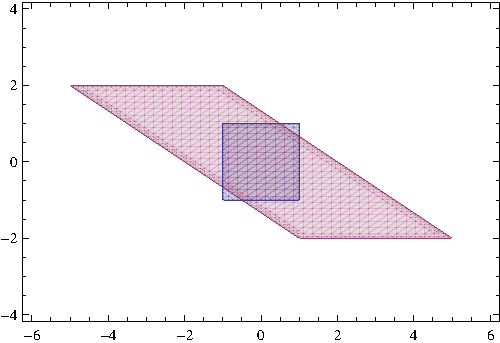
\includegraphics[width=\columnwidth]{infty.pdf}%
\end{figure}
\end{column}
\end{columns}
\begin{block}{В общем случае}
$$
\|\A\|_\infty = \max_i \sum_j |a_{ij}|
$$
\end{block}
}

\myframe{Матричная норма $\|\cdot\|_1$}
{
\begin{columns}[T]
\begin{column}{0.6\textwidth}
Точка 
$\x = \left(\begin{smallmatrix}
	0\\1
\end{smallmatrix}\right)$
 с нормой $\|\x\|_1 = 1$ переходит в точку $$\y = \A\x = \begin{pmatrix}
	-3\\2
\end{pmatrix}$$
 с нормой $\|\y\|_1 = 5$. 

Для остальных точек $\|\x\|_1 = 1$ 
$$\|\A\x\|_1 \leq 5$$
$$
\|\A\|_1 = 5
$$
\end{column}

\begin{column}{0.4\textwidth}
$$
\A = \begin{pmatrix}
	2&-3\\
	0&2
\end{pmatrix}
$$
\begin{figure}%
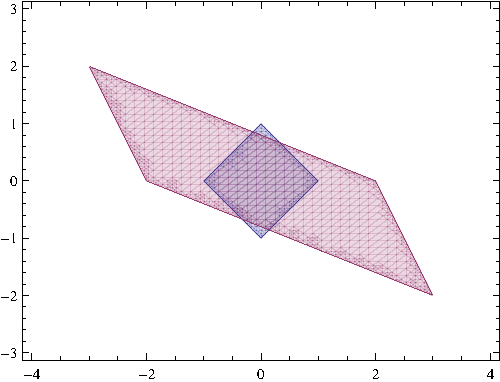
\includegraphics[width=\columnwidth]{l1.pdf}%
\end{figure}
\end{column}
\end{columns}
\begin{block}{В общем случае}
$$
\|\A\|_1 = \max_j \sum_i |a_{ij}| = \|\A^T\|_\infty
$$
\end{block}
}

\myframe{Матричная норма $\|\cdot\|_E$}
{
\begin{columns}[T]
\begin{column}{0.6\textwidth}
Точка 
$\x = \frac{1}{\sqrt{5}}\left(\begin{smallmatrix}
	-1\\2
\end{smallmatrix}\right)$
 с нормой $\|\x\|_E = 1$ переходит в точку $$\y = \A\x = \frac{1}{\sqrt{5}}\begin{pmatrix}
	-8\\4
\end{pmatrix}$$
 с нормой $\|\y\|_E = 4$. 

Для остальных точек $\|\x\|_E = 1$ 
$$\|\A\x\|_E \leq 4$$
$$
\|\A\|_E = 4
$$
\end{column}

\begin{column}{0.4\textwidth}
$$
\A = \begin{pmatrix}
	2&-3\\
	0&2
\end{pmatrix}
$$
\begin{figure}%
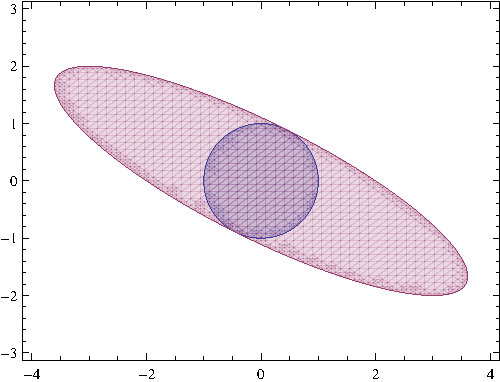
\includegraphics[width=\columnwidth]{euclid.pdf}%
\end{figure}
\end{column}
\end{columns}
\begin{block}{В общем случае}
$$
\|\A\|_E = \sqrt{\max \lambda(\A^T\A)}
$$
\end{block}
}

\myframe{Матричная норма $\|\cdot\|_E$}
{
	Докажем, что $\|\A\|_E = \sqrt{\max \lambda(\A^T\A)}$.
	$$
	\|\A\x\|_E = \sqrt{(\A\x,\A\x)} = \sqrt{\x^T\A^T\A\x} = \sqrt{(\x,\A^T\A\x)}
	$$
	\pause
	Матрица $\A^T\A$ симметрична и положительно определена. Значит у нее 
	существует ортонормированный базис из собственных векторов, 
	причем все собственные числа неотрицательны
	$$
	\A^T\A \x_k = \lambda_k \x_k, \quad \lambda_k \geq 0
	$$
}

\myframe{Матричная норма $\|\cdot\|_E$}
{
	$$
	\A^T\A \x_k = \lambda_k \x_k, \quad \lambda_k \geq 0
	$$
	Разложим $\x$ по этому базису $\left\{\x_k\right\}$
	\begin{align*}
	\x = \sum_k \alpha_k \x_k\\
	\A^T\A\x = \A^T\A \sum_k \alpha_k \x_k = \sum_k \alpha_k \lambda_k \x_k
	\end{align*}
	Учитывая, что базис ортонормированный $(\x_k,\x_m) = \delta_{km}$
	$$
	\left(\x,\A^T\A\x\right) = \sum_k \lambda_k \alpha_k^2 \leq \max_k \lambda_k \sum_k \alpha_k^2 = \left(\x,\x\right) \max_k \lambda_k 
	$$
	Возвращаясь к норме $\A\x$
	$$
	\|\A\x\|_E = \sqrt{(\x,\A^T\A\x)} \leq \sqrt{\max \lambda(\A^T\A)} \sqrt{(\x,\x)} = \sqrt{\max \lambda(\A^T\A)}
	$$
}

\myframe{Матричная норма $\|\cdot\|_E$}
{
	$$
	\|\A\x\|_E = \sqrt{(\x,\A^T\A\x)} \leq \sqrt{\max \lambda(\A^T\A)} \sqrt{(\x,\x)} = \sqrt{\max \lambda(\A^T\A)}
	$$
	Покажем, что норма $\|\A\|_E$ не может быть меньше $\sqrt{\max \lambda(\A^T\A)}$. Действительно, норма должна удовлетворять
	$$
	\|\A\|_E = \|\A\|_E \|\x_k\|_E \geq \|\A \x_k\|_E = \sqrt{(\x_k, \A^T\A \x_k)}= \sqrt{\lambda_k}
	$$
	Таким образом,
	$$
	\sqrt{\lambda_k} \leq \|\A\|_E \leq \sqrt{\max_k \lambda_k}
	$$
	Последнее возможно только при
	$$
	\|\A\|_E = \sqrt{\max_k \lambda_k}
	$$
}

\myframe{Матричная норма $\|\cdot\|_E$}
{
	Еще раз вернемся к матрице 
	$$
	\A = \begin{pmatrix}
		2&-3\\
		0&2
	\end{pmatrix},\qquad
	\A^T\A = \begin{pmatrix}
		4&-6\\
		-6&13
	\end{pmatrix}
	$$
	Собственные числа матрицы $\A^T\A$: $\lambda_1 = 1, \lambda_2 = 16$, ортонормированные собственные вектора
	$$
	\x_1 = \frac{1}{\sqrt{5}}\begin{pmatrix}
		2\\1
	\end{pmatrix}, \quad
	\x_2 = \frac{1}{\sqrt{5}}\begin{pmatrix}
		-1\\2
	\end{pmatrix}, \quad	
	$$
	$$
	\|\A\|_E = \sqrt{16} = 4
	$$
	Особенно просто норма $\|\cdot\|_E$ вычисляется в случае $\A = \A^T$
	$$
	\|\A\|_E = \sqrt{\max\lambda(\A^T\A)} = \sqrt{\max\lambda(\A^2)} = \max|\lambda(\A)|
	$$
}

\section{Обусловленность}
\myframe{Фиксированная правая часть}
{
	Рассмотрим систему 
	$$
	\A\x = \b
	$$
	и ``близкую'' к ней систему
	$$
	\A(\x+\delta \x) = \b + \delta \b
	$$
	Оценим относительную погрешность решения
	$$
	\frac{\|\delta\x\|}{\|\x\|} \leq \frac{\|\A^{-1}\|\|\delta \b\|}{\|\x\|} =
	\frac{\|\A^{-1}\|\|\delta \b\|}{\|\A^{-1}\b\|} =
	\frac{\|\A^{-1}\|\|\b\|}{\|\A^{-1}\b\|}\frac{\|\delta \b\|}{\|\b\|}
	$$
	Обозначим $\nu(\A,\b) = \frac{\|\A^{-1}\|\|\b\|}{\|\A^{-1}\b\|}$
	\begin{block}{}
	$$\frac{\|\delta\x\|}{\|\x\|} \leq \nu(\A,\b) \frac{\|\delta \b\|}{\|\b\|}$$
	\end{block}
}

\myframe{Фиксированная правая часть}
{
	\begin{block}{}
	$$\frac{\|\delta\x\|}{\|\x\|} \leq \nu(\A,\b) \frac{\|\delta \b\|}{\|\b\|}, \quad \nu(\A,\b) = \frac{\|\A^{-1}\|\|\b\|}{\|\A^{-1}\b\|}$$
	\end{block}
	Поскольку $\|\A^{-1}\b\| \leq \|\A^{-1}\|\|\b\|$
	$$
	\nu(\A,\b) \geq 1,
	$$
	причем существует такая правая часть $\b$, что $\nu(\A,\b) = 1$. Это именно то значение $\b$, при котором
	$$
	\| \A^{-1} \b \| = \|\A^{-1}\| \|\b\|
	$$
	При этом относительная погрешность решения не превосходит относительную погрешность правой части
}

\myframe{Произвольная правая часть}
{
	Посмотрим, какой может быть величина $\nu(\A,\b)$ в зависимости от $\b$. С одной стороны,
	$$
	\nu(\A,\b) = \frac{\|\A^{-1}\|\|\b\|}{\|\A^{-1}\b\|} \geq 1
	$$
	Введем
	$$
	\mu(\A) = \max_{\b} \nu(\A, \b)
	$$
	$$
	\mu(\A) = \|\A^{-1}\|\max_{\b} \frac{\|\b\|}{\|\A^{-1}\b\|} = \|\A^{-1}\|\max_{\x} \frac{\|\A\x\|}{\|\x\|} = \|\A^{-1}\| \|\A\|
	$$
	Таким образом, для произвольной правой части
	\begin{block}{}
	$$\frac{\|\delta\x\|}{\|\x\|} \leq \mu(\A) \frac{\|\delta \b\|}{\|\b\|}, \quad \mu(\A) = \|\A\|\|\A^{-1}\|$$
	\end{block}	
}

\myframe{Число обусловленности}
{
	Число $\mu(\A)$ называется обусловленностью матрицы $\A$ и показывает,
	насколько матрица ``близка'' к вырожденной. Поскольку
	$$
	\mu(\A) \geq \nu(\A,\b) \geq 1,
	$$
	относительная погрешность решения никогда не меньше относительной погрешности правой части. Более того, для любой матрицы $\A$ 
	можно найти такие $\b$ и $\delta \b$, что относительная погрешность решения будет ровно в $\mu(\A)$ раз больше относительной
	погрешности правой части.
	
	Эта погрешность связана с самой задачей решения СЛАУ, а не с конкретным методом ее решения, и ни один численный метод
	не может решить эту задачу точнее. Поэтому данная погрешность называется \emph{неустранимой}
}

%%%%%%%%%%%%%%%%%%%%%%%%%%%%%%%%%%%%%%%%%%%%%%%
%%%%%%%%%%%%%%%%%%%%%%%%%%%%%%%%%%%%%%%%%%%%%%%
%%%%%%%%%                            %%%%%%%%%%
%%%%%%%%%%%%%%%%%%%%%%%%%%%%%%%%%%%%%%%%%%%%%%%
%%%%%%%%%%%%%%%%%%%%%%%%%%%%%%%%%%%%%%%%%%%%%%%
{
\setbeamertemplate{headline}[default] 
\frame{
	\begin{center}
	{\Huge Спасибо за внимание!}
	\end{center}
	\bigskip
	\begin{center}
	{\color{blue}{tsybulin@crec.mipt.ru}}
	\end{center}
	}
}

\end{document}
